\documentclass{article}
\usepackage{amsmath,amssymb,setspace,verbatim,graphicx,enumerate,enumitem}
\usepackage[top=1in,bottom=1in,left=1in,right=1in,nohead,nofoot]{geometry}
\usepackage{caption}
% \usepackage{subcaption}
% \usepackage{subfig}
% \usepackage{subfloat}
% \usepackage{tabularx}
\usepackage{mdframed}

\newenvironment{Rcode}% environment name 
{%begin code
    \begin{mdframed}
    \#R code
    \begin{small}
}
{%end code
    \end{small}
    \end{mdframed}
}

\newenvironment{console}% environment name 
{%begin code
    \begin{mdframed}
    \#Console
    \begin{small}
}
{%end code
    \end{small}
    \end{mdframed}
}

% \parindent 0in
% \parskip .2in
% \pagestyle{empty} \singlespacing
% %\newcommand{\vect}[1]{\mbox{\boldmath $ #1$}}
% \newcommand{\bv}[1]{\mathbf{#1}}
% \setlist{noitemsep,topsep=0pt,parsep=0pt,partopsep=0pt}


\begin{document}
\title{FDA Homework 1}
\author{Seokjun Choi}
\date{September 30, 2019}
\maketitle

\section{Chapter 1}
\subsection{Problem 1}

\textbf{
The pinch is a dataset included in the fda package. It consists of 151 measurements of pinch force for 20 replications (curves). 
}
\subsubsection*{(a)  Convert the pinch data to functional objects using 15 B-splines of order four (cubic splines) and plot the 20 smoothed curves on one graph.}
To get the result we want, call the fda package and execute the code below.

\begin{Rcode}
    \begin{verbatim}
b_spline_basis<-create.bspline.basis(c(1,151), nbasis=15, norder=4)
pinch.F<-Data2fd(1:151, pinch, b_spline_basis)
plot(pinch.F)
    \end{verbatim}
\end{Rcode}
Then we get the result.
\begin{figure}[hh]
    \centering
    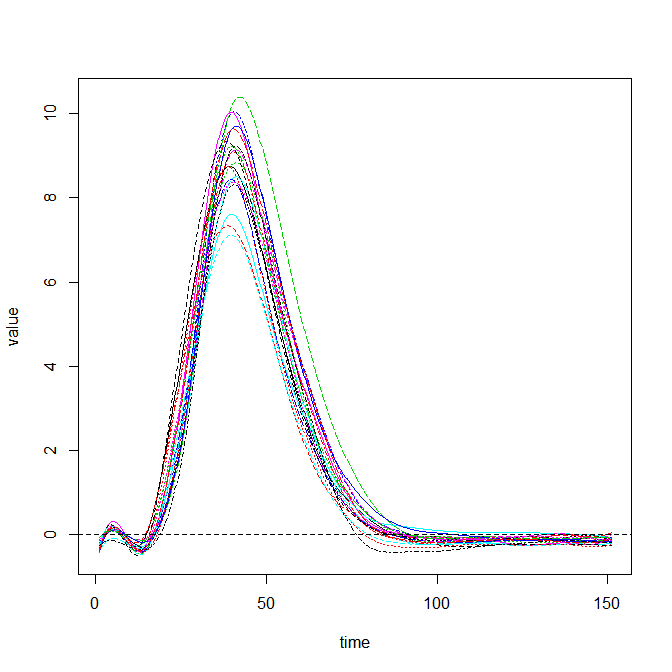
\includegraphics[height=8cm]{pinch_F_plot.png}
    \caption{fitting pinch data using 15 b-splines}
\end{figure}

\newpage
\subsubsection*{(b) Calculate the pointwise mean and SD and add them to the plot.}
For calculation, run the code below.
\begin{Rcode}
    \begin{verbatim}
pinch.F.mean <- mean(pinch.F)
pinch.F.mean$coefs

pinch.F.std <- std.fd(pinch.F)
pinch.F.std$coefs

par(mar=c(4,4,1,1))
plot(pinch.F, col="grey")
plot(pinch.F.mean,lwd=4,add=TRUE)
plot(pinch.F.std, lwd=4, add=TRUE, col="red")
    \end{verbatim}
\end{Rcode}

For analytic expression of pointwise mean and point sd, denote $b_i$ as i-th b-spline of order 4
on domain $[0,120] \subset \Re$. Then
\[Mean(x)=\sum_{i=1}^{16}c_ib_i(x)\]
\[Sd(x)=\sum_{i=1}^{16}s_ib_i(x)\]
where $c_i$ : -0.31109576, 0.73142704, -1.63349675, 2.72475346, 10.93667264, 6.03218354, 2.28791198, 0.34957598, -0.09607592, -0.16637125, -0.11240041, -0.15664938, -0.10293668, -0.16311715, -0.11897440
\\
and $s_i$ : 0.0846463, 0.1182031, -0.0996403, 0.9735739, 0.6517423, 1.1140145, 0.5002106, 0.3255844, 0.1166337, 0.1232983, 0.0639047, 0.0869009, 0.0824064 0.0776430, 0.07207136
respectively. 

And here is a plot of the result.
\begin{figure}[hh]
    \centering
    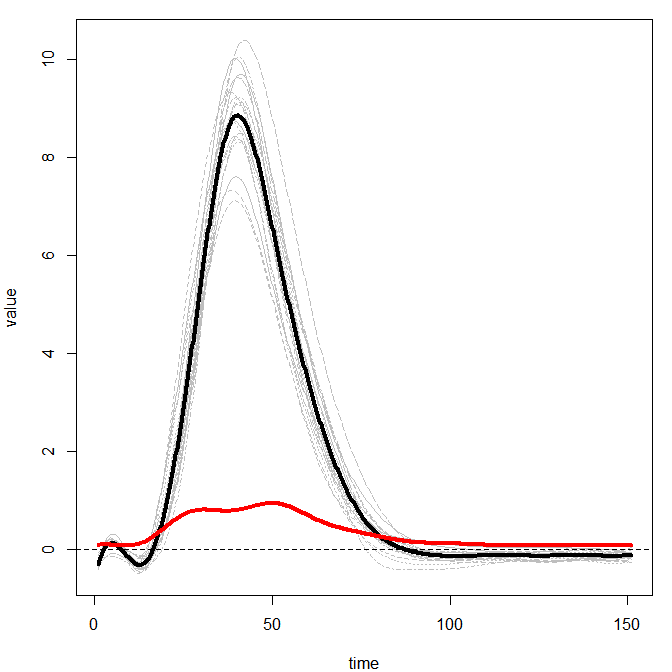
\includegraphics[height=8cm]{pinch_F_mean_var_plot.png}
    \caption{fitting pinch data using 15 b-splines: \\ Black bold curve is mean, and red bold curve is standard deviation.}
\end{figure}


\newpage
\subsubsection*{(c) Graph the perspective and contour plots of the sample covariance function $\hat{c}(t,s)$ of the pinch curves.}

We can easily do them by using for var.fd function of fda package and persp, contour function of R.
\begin{Rcode}
    \begin{verbatim}
pinch.F.cov <- var.fd(pinch.F)
dim(pinch.F.cov$coef) #15*15
grid <- 1:15
pinch.F.cov.mat = eval.bifd(grid, grid, pinch.F.cov)
par(mfrow=c(1,2), mar=c(4,4,1,1))
persp(grid, grid, pinch.F.cov.mat, xlab="s", ylab="t", zlab="cov(s,t)")
contour(grid, grid, pinch.F.cov.mat)
    \end{verbatim}
\end{Rcode}

Result plots are here.

\begin{figure}[hh]
    \centering
    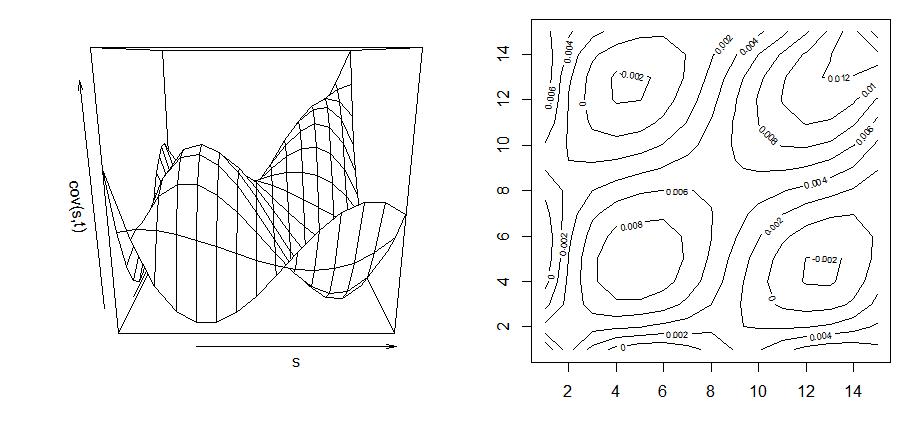
\includegraphics[height=8cm]{pinch_F_cov_persp_contour_plot.png}
    \caption{fitting pinch data using 15 b-splines: \\ covariance perspective plot and contour plot.}
\end{figure}

\newpage
\subsubsection*{(d) Graph the first four EFPC’s of the pinch data. How many components do you need to explain 90\% of variation?}

Let's do PCA with 4 components following the instruction of problem, and see the proportions of variance of each component for determining number of components for 90\% explanation.

\begin{Rcode}
    \begin{verbatim}
par(mfrow=c(1,1))
pinch.F.pca = pca.fd(pinch.F, nharm=4)
plot(pinch.F.pca$harmonics, lwd=3)
pinch.F.pca$varprop
    \end{verbatim}
\end{Rcode}

Firstly, I'll plot the first 4 eigenfunctions.

\begin{figure}[hh]
    \centering
    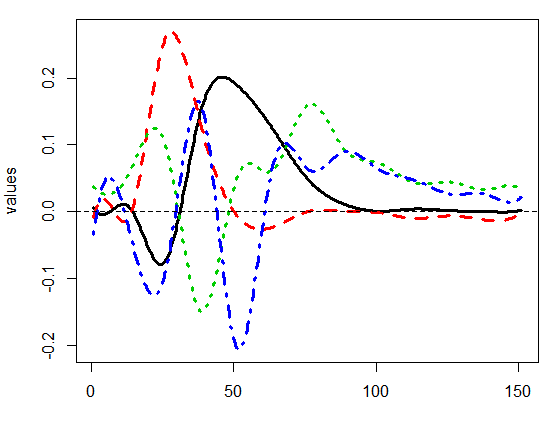
\includegraphics[height=8cm]{pinch_F_pca_4components_plot.png}
    \caption{fitting pinch data using 15 b-splines and do PCA: \\ first 4 components.}
\end{figure}

And the ouput of last line is

\begin{console}
    \begin{verbatim}
> pinch.F.pca$varprop
[1] 0.67225632 0.24845297 0.04603548 0.01933904
    \end{verbatim}
\end{console}

Since the sum of first 2 proportion is 0.9207093, we need only 2 components to reach 90\% level of explanation of variation.


\newpage
\subsection{Problem 2}
\textbf{
For this problem, download the R package fds and use the data set of the United States Federal Reserve interest rates, FedYieldcurve,
which contains the monthly interest rates from January 1982 to June 2009.
The x-values are the maturity terms of 3, 6, 12, 60, 84 and 120 months which can be identified with the $t_j$ in this chapter.
The y-values are the interest rate of the United States Treasury obligations due in x months which can be identified with the $x_n(t_j)$,
where n is a month in the range January 1982 to June 2009.}

Firstly Note that, in R code, after \'fds\', \'fda\' libraries are called, variable names are set by
\begin{Rcode}
    \begin{verbatim}
yield = FedYieldcurve
terms = yield$x
    \end{verbatim}
\end{Rcode}


\subsubsection*{(a) On one graph, plot the interest rates $x(t_j)$ for January 1982 and for June 2009 against the maturity terms $t_j$. How do the interest rates in these two months compare?}
Run the code below and get a plot before discuss about comparing yield rates.
\begin{Rcode}
    \begin{verbatim}
plot(terms, yield$y[,1], pch=15, ylab="Yield", ylim=c(0,16)) 
points(terms, yield$y[,330], pch=16)
    \end{verbatim}
\end{Rcode}
\begin{figure}[hh]
    \centering
    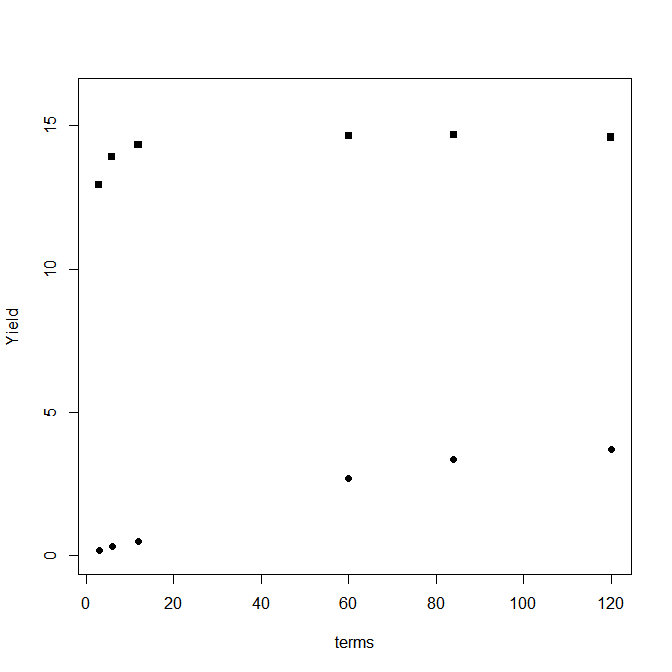
\includegraphics[height=8cm]{yield_2terms.png}
    \caption{yield points of Jan 1982 and June 2009}
\end{figure}
At the maturity of the data exist, we can compare yield rates directly by calculating square sum of difference, or supremum of absolute value of difference.
But for other maturity values which are not at datapoint, 
we should use more than data themself. We may use interpolation technique, or other fitting method like LSE or time series analysis's,
but since here are FDA class, we may use method of FDA's! :)

\newpage
\subsubsection*{(b) Convert the yield data to functional objects using bspline basis with four basis functions. 
Calculate and plot the the mean yield function. What is the average behavior of interest rates as a function of the maturity?}

Execute the code below for following the first and second directions of problem.
\begin{Rcode}
    \begin{verbatim}
b_spline_basis = create.bspline.basis(c(1,120), nbasis=4)
yield.F = Data2fd(terms, yield$y, b_spline_basis)
plot(yield.F, col='gray')

yield.F.mean = mean(yield.F)
plot(yield.F.mean,lwd=4,add=TRUE)
    \end{verbatim}
\end{Rcode}
The result plot is,\\
\begin{figure}[hh]
    \centering
    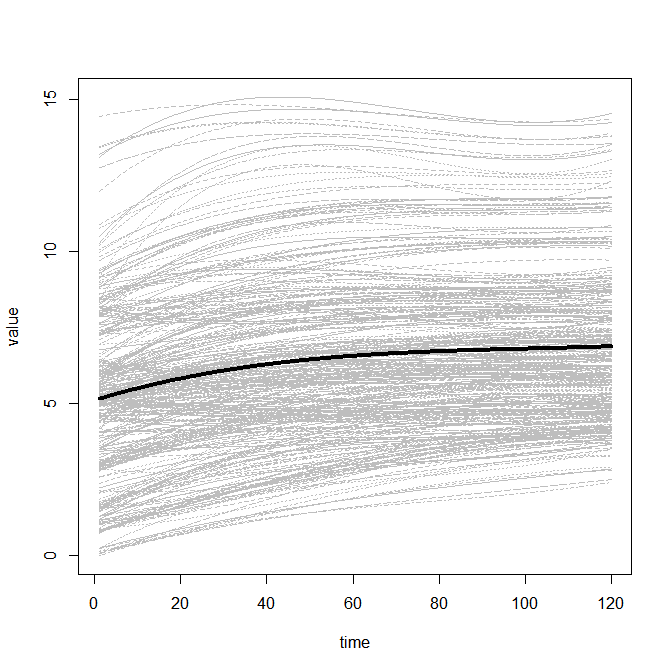
\includegraphics[height=8cm]{yield_bspline4fit}
    \caption{Fitting yield data using b-spline 4 basis:\\Bold curve indicates mean.}
\end{figure}

The mean curve has increasing shape generally, but the slope goes flatter with maturity becoming longer.

\newpage
\subsubsection*{(c) Plot the first principal component of the interest rate curves. What percentage of variance does this component explain? Interpret the plot and the percentage of variance.}
Run the below code to perform PCA with one component.
\begin{Rcode}
    \begin{verbatim}
yield.F.pca = pca.fd(yield.F, nharm=1)
plot(yield.F.pca$harmonics, lwd=3, , ylim=c(-1,1))
yield.F.pca$varprop
    \end{verbatim}
\end{Rcode}

The second line gives the plot of the component function.
\begin{figure}[hh]
    \centering
    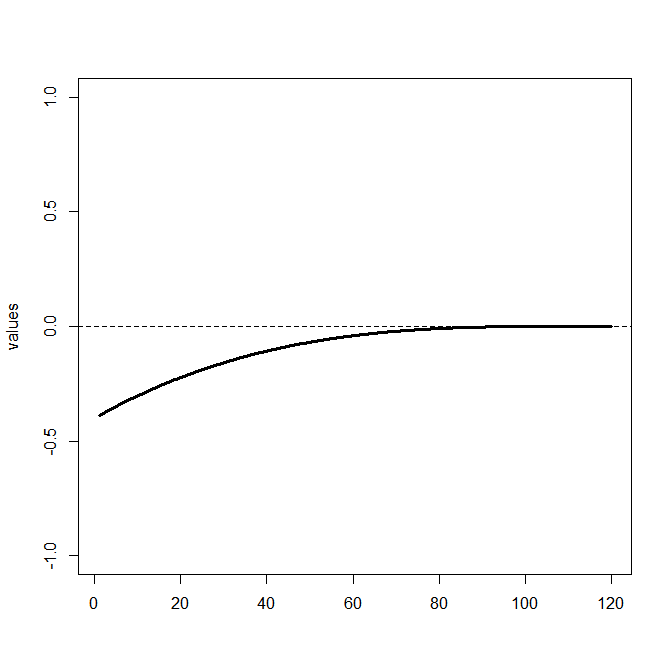
\includegraphics[height=8cm]{yield_bspline4fit_pca_1comp.png}
    \caption{Fitting yield data using b-spline 4 basis:\\ First component of pca.}
\end{figure}

Since overall fitted functions have similar form as we view at Figure 6, the shape of the component also has similar shape to them, especially to the mean curve.

\begin{console}
    \begin{verbatim}
> yield.F.pca$varprop
[1] 0.999982
    \end{verbatim}
\end{console}

Likewise, the proportion of explained variation has high value, consisting the above context.

\newpage
\subsection{Problem 6}
\textbf{
In this section we expressed \(x_n(t)=\sum_{m=1}^{M}c_{nm}B_m(t)\). One can show that
\[\bar{x}_N(t)=\sum_{m=1}^{M}a_mB_m(t) \]
and
\[\hat{c}(t,s)=\sum_{m=1}^{M}\sum_{k=1}^Mb_{mk}B_m(t)B_k(s)\]
Find expressions for the coefficients $a_m$ and $b_{mk}$ assuming that the
$B_m(t)$ are an orthonormal basis:
\[\int B_m(t)B_k(t)=1_{m=k}\]
}
\\

Happily, there is solution of these problems in our lecture note, so I repeat the contents.\\
Firstly for sample mean, observe that
\[\bar{x}_N(t)=\frac{1}{N}\sum_{n=1}^{N}x_n=\frac{1}{N}\sum_{n=1}^{N}\sum_{m=1}^{M}c_{nm}B_m(t)=\sum_{m=1}^{M}(\frac{1}{N}\sum_{n=1}^{N}c_{nm})B_m(t)\]
so if we set \(a_m=\frac{1}{N}\sum_{n=1}^{N}c_{nm}\), we get the expression that we want.\\
And for sample covariance,
\[\hat{c}(t,s)=\frac{1}{N-1}\sum_{n=1}^{N}(x_n(t)-\bar{x}(t))(x_n(s)-\bar{x}(s))\]
then where \(\tilde{c}_{nm}=c_{nm}-a_m\),
\[=\frac{1}{N-1}\sum_{n=1}^{N}\sum_{m=1}^{M}\sum_{k=1}^{M}\tilde{c}_{nm}\tilde{{c}}_{nk}B_{m}(t)B_{k}(s)\]
\[=\sum_{m=1}^{M}\sum_{k=1}^{M}(\frac{1}{N-1}\sum_{n=1}^{N}\tilde{c}_{nm}\tilde{{c}}_{nk})B_{m}(t)B_{k}(s)\]
so if we set \(b_{mk}=\frac{1}{N-1}\sum_{n=1}^{N}\tilde{c}_{nm}\tilde{{c}}_{nk}\), 
or equivalently using matrix notation if we set \(b_{mk}=(N-1)^{-1}(\mathbf{\tilde{c}}^T\mathbf{\tilde{c}})_{mk}\), we get what we want.



\newpage
\section{Chapter 2}
\subsection{Problem 1}
Verify the equality,
\[\int_{0}^{T}[L(x)(t)]^2dt=\pi\omega^5\sum_{j=2}^{J}j^2(j^2-1)^2(a_j^2+b_j^2)\]
with harmonic acceleration operator \(L(X)(t)=\omega^2x^{(1)}(t)+x^{(3)}(t), \omega=2\pi/T\) \\
and Fourier basis \(x_{J}(t)=c_0+\sum_{j=1}^{J}\{a_j\sin{\omega jt}+b_j\cos{\omega jt}\}\)

For a start, I'll calculate $x^{(i)}(t), i=1,3$. For notational simplicity, I omit subscript J. The results are
\[x^{(1)}(t) = \sum_{j} \{a_j\omega j \cos{\omega jt} - b_j\omega j \sin{\omega jt}\}\]
\[x^{(3)}(t) = \sum_{j} \{-a_j\omega^3 j^3 \cos{\omega jt} + b_j\omega^3 j^3 \sin{\omega jt}\}\]
I notice that when j=1, L become 0 operator. So we can exclude to j=1 case in summation. \\
Then, our operator are actually
\[L(x)(t)=\sum_{j}\{a_j\omega^3(j-j^3)\cos{(wjt)} + i\frac{1}{i}b_j\omega^3(j^3-j)\sin(wjt)\}\]
Then, using definition of complex sine and cosine function, we can rewrite L as
\[L(x)(t)=\sum_{j}\sqrt{\frac{(a_j+b_j)^2\omega^6j^2(j^2-1)^2}{2}}e^{i\omega jt}\]
Then, above form can be seen as formal Fourier expansion form (on a circle $[0,T(=2\pi/\omega)]$). So, by Parseval's identity,
\[\frac{\omega}{2\pi} \int_{0}^{T}|L(x)(t)|^2dt = \frac{1}{2}\sum_{j}(a_j+b_j)^2\omega^6j^2(j^2-1)^2\]
Multiplying $\frac{2\pi}{\omega}$ to both hand terms, we get the equation which we want.


\newpage
\subsection{Problem 2}
\textbf{
Proceed with FedYieldcurve data, which contains the monthly Federal Reserve interest rates, cf. Problem 1.6.2.
}

Likewise at problem 2 of chapter 1, firstly I set the variables like this of R code after call libraries.
\begin{Rcode}
    \begin{verbatim}
yield.J1982 = FedYieldcurve$y[,1]
terms = FedYieldcurve$x
    \end{verbatim}
\end{Rcode}


\subsubsection*{(a) Smooth the interest rates (yields) in January 1982 using a B–spline basis 
with four basis functions. Plot the raw and smoothed interest rates on one graph.}

FedYieldcurve data are monthly, so we proceed with only one curve.
To get the plot of raw and fitted curves with 4 b-splines, run this code.
\begin{Rcode}
    \begin{verbatim}
b_spline_basis4 = create.bspline.basis(c(1,120), nbasis=4)
yield.F4 = Data2fd(terms, yield.J1982, b_spline_basis4)
plot(yield.F4, col='black', xlim=c(0,120), ylim=c(12.5,15.5), 
    xlab="maturity", ylab="yield rate")
points(terms, yield.J1982, type='l', col='gray')
    \end{verbatim}
\end{Rcode}
The result is here.
\begin{figure}[hh]
    \centering
    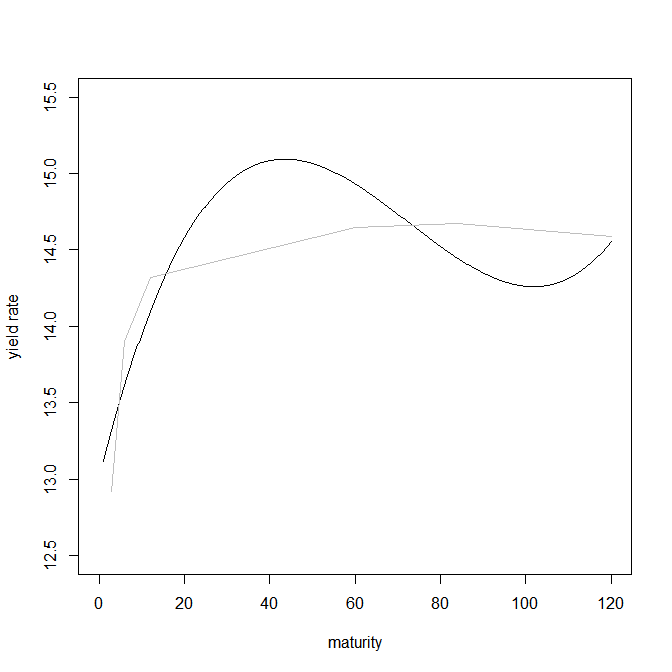
\includegraphics[height=8cm]{1982Jyield_raw_bspline4.png}
    \caption{January 1982 yield:\\ gray line is raw data, and black curve is fitted curve using 4 b-splines.}
\end{figure}


\newpage
\subsubsection*{(b) Re-fit the January 1982 yields using a penalized smoothing based on six basis functions 
(as many as data points) with the smoothing parameter $\lambda = 1$, 
and the second derivative as the penalty operator. Add the smooth in red to the graph you obtained 
in part (a) and comment on the result.}

By modifying just parameter of above code and adding smoothing code, we can get the results which we want.
\begin{Rcode}
    \begin{verbatim}
b_spline_basis6 = create.bspline.basis(c(1,120), nbasis=6)
par.F6.S1 = fdPar(b_spline_basis6, Lfdobj=2, lambda=1)
yield.F6.S1 = smooth.basis(terms, yield.J1982, par.F6.S1)

par(new=T)
plot(yield.F6.S1, xlim=c(0,120), ylim=c(12.5,15.5), ylab="", xlab="", col='red')
    \end{verbatim}
\end{Rcode}

Then we get below plot.

\begin{figure}[hh]
    \centering
    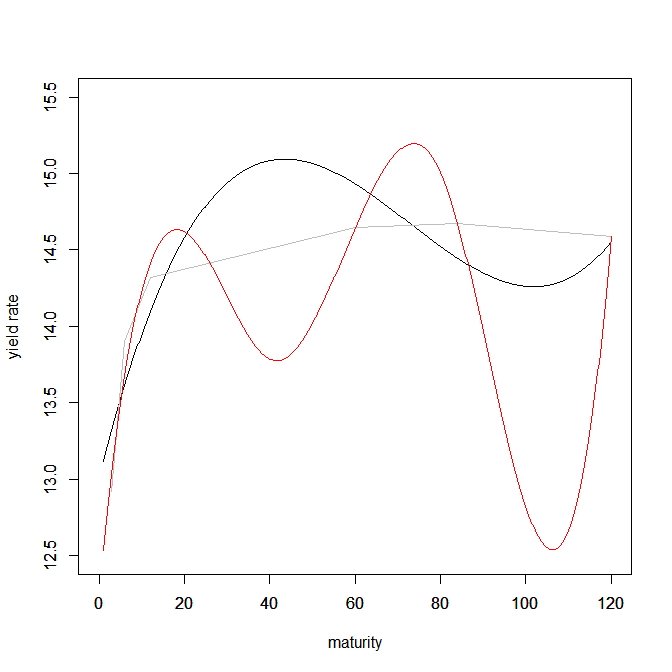
\includegraphics[height=8cm]{1982Jyield_raw_bspline4_bspline6.png}
    \caption{January 1982 yield: \\ gray: raw data \\ black : fitted curve using 4 b-splines \\ red : fitted curve using 6 b-splines.}
\end{figure}

Since the number of basis increases and we are using polynomial basis, the fitted curve with 6-basis has more variation,
and consquently it seems to get worse comparing with (a)'s 4 basis case to explain original (raw) line (in fact, points). 
This phenomenon is similar to the outcome of typical overfitting cases raised by too high order polynomial model for fitting to small (point) dataset.
And at our functional data case where the order consists the number of basis, above result consists with our intuition.
(Note that although here, the functional analysis, is the term "order" which means other things that i.e. the (polynomial) order of each b-spline,
so statement like above may make some confusing, but I think an increasing of 'the order' of each b-splines also gives similar effect and yields similar conclusion,
'intuitively' the statement still has some consistence with too-high-basis-number case like above.)

\newpage
\subsubsection*{(c) Repeat part (b) with several other smoothing parameters $\lambda$. Which $\lambda$ gives the most informative smooth curve?}

For finding enoughly best $\lambda$ value to satisfiablely most(?) informative smooth curve,
I will consider candidates of $\lambda$ value which are integers from 1 to 200. 
(For 'the most', we should explore more deliberately including floating number, but I'll skip this for simplicity, and just take an integer value.)
And as a criterion, I will calculate GCVs - a kind of validation measure for fitting - for each $\lambda$ cases,
and choose a $\lambda$ value which gives the lowest GCV value. \\
run the below code.
\begin{Rcode}
    \begin{verbatim}
candid_lambda = seq(1, 200, 1)
gcvs = rep(0, length(candid_lambda))
for(i in 1:length(candid_lambda)){
    par.F6.Si = fdPar(b_spline_basis6, Lfdobj=2, lambda=candid_lambda[i])
    yield.F6.Si = smooth.basis(terms, yield.J1982, par.F6.Si)
    gcvs[i]=mean(yield.F6.Si$gcv)
}
plot(candid_lambda, gcvs)
which.min(gcvs)
    \end{verbatim}
\end{Rcode}
The second line from the end gives plot of GCV values for each $\lambda$ value, and
the output of last line give best $\lambda$ value to us.

\begin{figure}[hh]
    \centering
    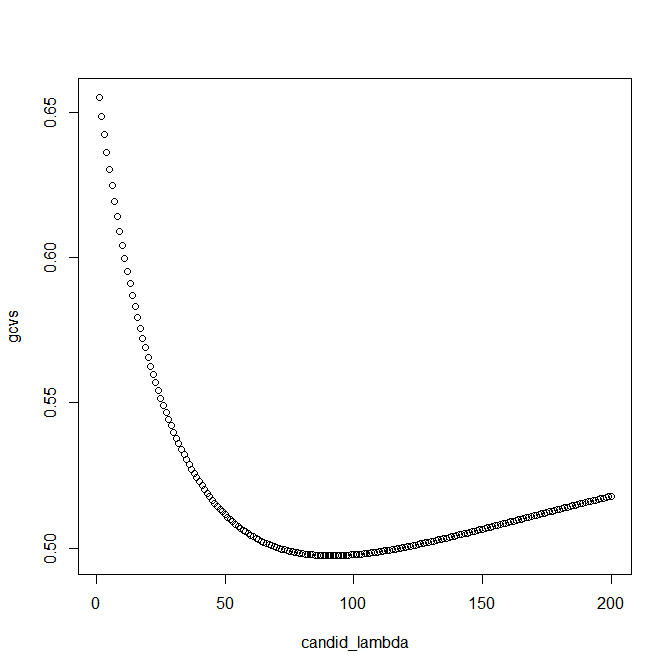
\includegraphics[height=8cm]{1982Jyield_bspline6_lambda_gcv.png}
    \caption{January 1982 yield: GCVs for each $\lambda$:\\ smoothed by penalized smoothing method with 2nd derivative operator, fitted using 6 b-splines.}
\end{figure}

And minimum GCV value is at $\lambda=91$. So, I'll repeat the smoothing and fitting procedure with the $\lambda=91$ value,
and get a fitted curve. Additionally, I'll plot second derivative curves for each. \\Run this code block.
\begin{Rcode}
    \begin{verbatim}
#take lambda=91
par.F6.S91 = fdPar(b_spline_basis6, Lfdobj=2, lambda=91)
yield.F6.S91 = smooth.basis(terms, yield.J1982, par.F6.S91)
plot(yield.F4, col='black', xlim=c(0,120), ylim=c(12.5,15.5))
points(terms, yield.J1982, type='l', col='gray')
par(new=T)
plot(yield.F6.S1, xlim=c(0,120), ylim=c(12.5,15.5), ylab="", xlab="", col='red')
par(new=T)
plot(yield.F6.S91, xlim=c(0,120), ylim=c(12.5,15.5), ylab="", xlab="", col='blue')

#for 2nd derivative
plot(deriv.fd(yield.F4), col='black', ylim=c(-0.1,0.4))
par(new=T)
plot(deriv(yield.F6.S1$fd), col='red', ylim=c(-0.1,0.4))
par(new=T)
plot(deriv(yield.F6.S91$fd), col='blue', ylim=c(-0.1,0.4))
    \end{verbatim}
\end{Rcode}

Then, we get below plots.

\begin{figure}[hh]
    \centering
    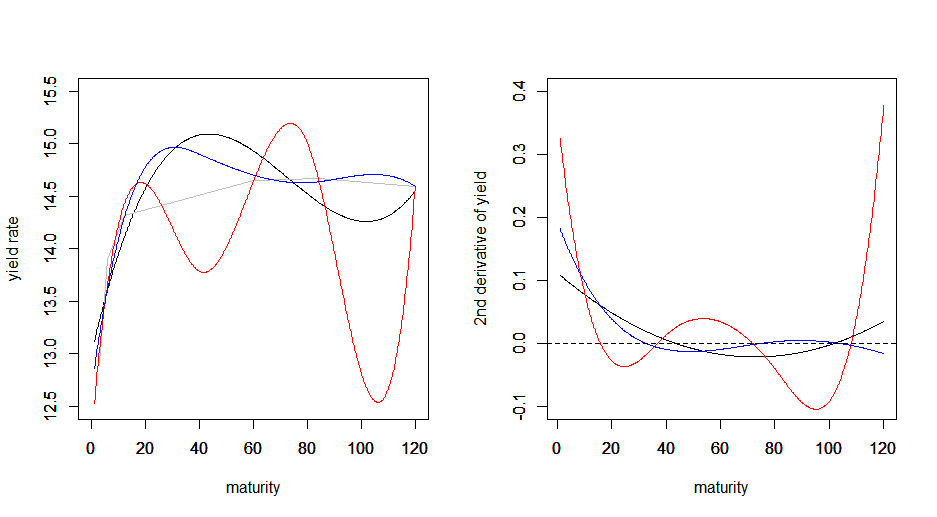
\includegraphics[height=8cm]{1982Jyield_comp_plot.png}
    \caption{January 1982 yield:\\
        \textbf{left: yield rate, right: 2nd derivative of yield rate}\\
        gray: original data (caution: no derivative curve)\\
        black: fitted using 4 b-spline basis\\
        red: fitted using 6 b-spline basis and smoothed with $\lambda=1$\\
        blue: fitted using 6 b-spline basis and smoothed with $\lambda=91$\\
        }
\end{figure}

On the plots, we can verify the effect of smoothing with chosen $\lambda=91$ value by watching blue curve.
On whole of maturity interval $[0,120]$, the blue curve of right plot, 2nd derivative of $\lambda=91$, has values closer to 0 comparing with red curve, of $\lambda=1$,
and also blue curve of left plot is better to explain original rate comparing to red one.
And Generally, on most part of domain interval, blue curve shows good performance as black curve which is fitted with 3 b-spline basis.

So, consquently, it is important to choose proper number of basis and smoothing parameter for explaining a given data well.



\newpage
\subsection{Problem 5}
\textbf{
In this problem, we will explore some potential dangers of curve alignment. 
A bump function centered at a value $c_0$, with radius $r_0$, and amplitude $a_0$ is defined as 
}
\begin{equation*}
    f(x) = \begin{cases}
        a_0\exp{\{-(1-(\frac{x-c_0}{r_0}^2)^{-1})\}} &\text{if } |x-c_0|<r_0 \\
        0 &\text{otherwise}
    \end{cases}
\end{equation*}
\subsubsection*{(a) Simulate a functional sample over the unit interval each with a sample size of 50 from the Mat\'{e}rn process. 
For the first half of the sample, set the mean function equal to the bump function with parameters $(c_0,r_0,a_0)=(3/8,1/4,5)$.
For the second half use $(c_0,r_0,a_0)=(5/8,1/4,5)$.
You may choose the values for the Mat\'{e}rn covariance function as well as the number of points sampled per curve.
Plot all of the curves and include a curve for the overall mean function.}

Following direction of problem, run this code and generate Mat\'{e}rn process and plot results.
As parameters of covariance of Mat\'{e}rn process, I choose $\sigma^2=1, \rho=0.1, \nu=0.5$ respectively,
and as number of points, I take 100 on $[0,1)$ (more exactly, see 'times' variable on the code).

\begin{Rcode}
    \begin{verbatim}
        
library(fields)
library(expm)
library(fda)

num.sample = 50

#define bump function
bump = function(x, c0, r0, a0){
    result = rep(0, length(x))
    for(i in 1:length(x)){
        if(abs(x[i] - c0) < r0){
            result[i] = a0*exp(-(1-((x[i]-c0)/r0)^2)^-1)
        }
    }
    return(result)
}

times = seq(0,0.99,0.01)
bumpval1 = bump(times, 3/8, 1/4, 5)
bumpval2 = bump(times, 5/8, 1/4, 5)
# plot(times, bumpval2)

#generate Matern process
mt.sig2 = 1 #pointwise variance
mt.rho = 0.1 #range parameter (how quickly falls off)
mt.nu = 1/2 #smoothness parameter

d_mat = abs(outer(times,times,"-"))
C_1 = apply(d_mat, c(1,2), FUN=Matern, range=mt.rho, nu=mt.nu)
C_1 = C_1*mt.sig2
C_1_sq = sqrtm(C_1)


MaternSamples = matrix(0, length(times), num.sample)
for(i in 1:num.sample){
    Z<-rnorm(length(times))
    MaternSamples[,i] = C_1_sq%*%Z
}

MtSample.group1 = MaternSamples[, 1:(num.sample/2)]
MtSample.group2 = MaternSamples[, (num.sample/2+1):num.sample]


# mean adjust
for(i in 1:(num.sample/2)){
    MtSample.group1[,i] = MtSample.group1[,i] + bumpval1
    MtSample.group2[,i] = MtSample.group2[,i] + bumpval2
}
adjMtSamples = cbind(MtSample.group1, MtSample.group2)


#plot after adjusted by bump function
par(mfrow=c(1,3))
plot(times,MtSample.group1[,1],type="n", ylim=c(-3,4))
for(i in 1:(num.sample/2)){
    points(times, MtSample.group1[,i],type="l", col="red")
    points(times, MtSample.group2[,i], type="l", col="blue")
}
points(times, bumpval1, type="l", col="red", lwd=3)
points(times, bumpval2, type="l", col="blue", lwd=3)
points(times, rowMeans(adjMtSamples[,1:(num.sample/2)]), type="l", col="yellow", lwd=3)
points(times, rowMeans(adjMtSamples[,(num.sample/2+1):num.sample]), type="l", col="green", lwd=3)
#
plot(times, bumpval1, type="l", col="red", lwd=3, ylim=c(-3,4))
points(times, bumpval2, type="l", col="blue", lwd=3)
points(times, rowMeans(adjMtSamples[,1:(num.sample/2)]), type="l", col="yellow", lwd=3)
points(times, rowMeans(adjMtSamples[,(num.sample/2+1):num.sample]), type="l", col="green", lwd=3)
#
plot(times,MtSample.group1[,1],type="n", ylim=c(-3,4))
for(i in 1:(num.sample)){
    points(times, adjMtSamples[,i],type="l", col="grey")
}
points(times, 0.5*(bumpval1+bumpval2), type="l", col="black", lwd=3)
points(times, rowMeans(adjMtSamples), type="l", col="yellow", lwd=3)
    \end{verbatim}
\end{Rcode}

Last code block gives plots for simulated process and mean of them.

\begin{figure}[hh]
    \centering
    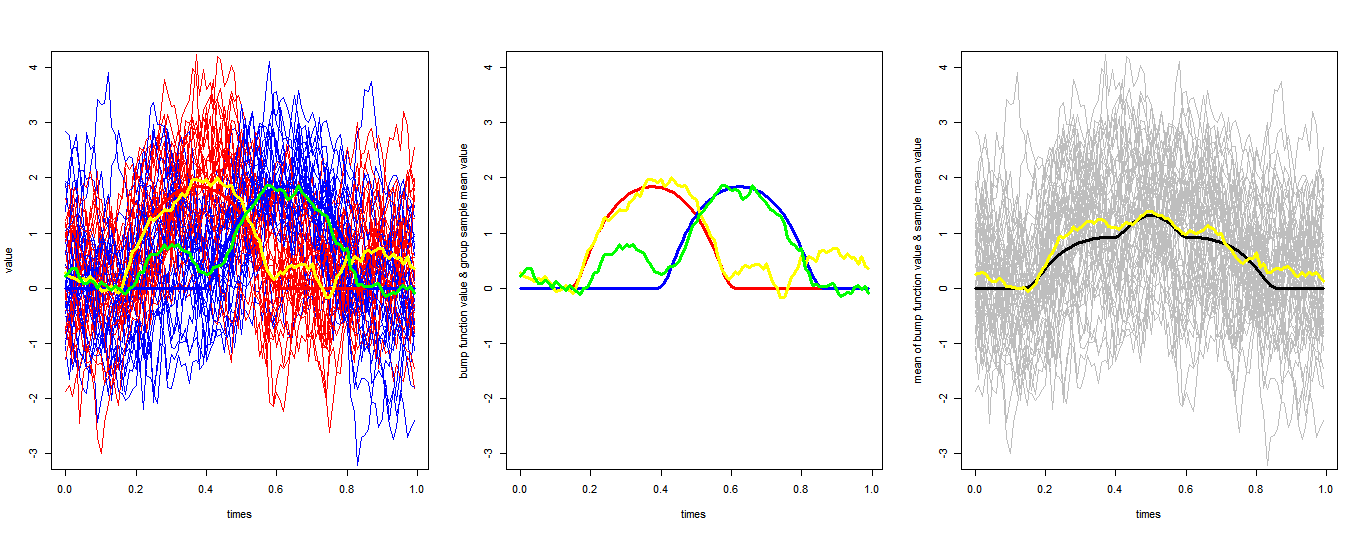
\includegraphics[height=6.3cm]{matern_verify_sim.png}
    \caption{Mat\'{e}rn process: generated samples\\(there is detailed information on body text.)}
\end{figure}

Each curve on result plots at below indicates,
\begin{itemize}
    \item{\textbf{left:} plot of whole processes with group infomation.\\
    red \& blue color indicates the group (first 25s \& last 25s) respectively.\\
    bold red \& blue curve are bump functions of groups. (group's theorical-population mean)\\
    and bold yellow and green curve are realized pointwise mean of each group. (group's sample mean)}
    \item{\textbf{middle:} draw only group mean curves from left one.}
    \item{\textbf{right:} plot of whole processes without group information.\\
    grey curves are 50 generated processes.\\
    bold black curve is mean of 2 bump functions. (theorical mean of total process)\\
    and bold yellow curve is mean of realized pointwise process. (total sample mean)}
\end{itemize}

By comparing sample mean curves to theorical one, we can see that simulated processes are properly generated to our purpose.


\newpage
\subsection*{(b) Align the curves using continuous registration. Plot the resulting curves and include a mean function. 
Comment on any differences with (a) and if the registered curves exhibit any odd patterns.}

Firstly, I do fitting process to get the functional object using 6 b-spline basis. (6 is arbitrarily chosen number.)
And next, I carry out the alignment procedure using continuous registration method.
Then finally, I plot the curves fitted of before and after the alignment.

Run the code below.
\begin{Rcode}
    \begin{verbatim}
# basic fitting to b-spline
b_spline_basis = create.bspline.basis(c(0,1), nbasis=6)
adjMtSample.f = smooth.basis(times, adjMtSamples, b_spline_basis)$fd

#plot: curves before alignment
par(mfrow=c(1,3))
plot(adjMtSample.f, ylim=c(-3,4), col='grey'); plot(mean(adjMtSample.f), add=T, lwd=3)

#apply continuous registration
adjMtSample.f.reg = register.fd(adjMtSample.f)

#plot: aligned curves
plot(adjMtSample.f.reg$regfd, col='grey', ylim=c(-3,4))
plot(mean(adjMtSample.f.reg$regfd), add=T, lwd=3, col='red')

#plot: compare only mean
plot(mean(adjMtSample.f), lwd=3, col='black', ylim=c(-3,4))
plot(mean(adjMtSample.f.reg$regfd), add=T, lwd=3, col='red')
    \end{verbatim}
\end{Rcode}

\newpage
Then, we get 3 plots,

\begin{figure}[hh]
    \centering
    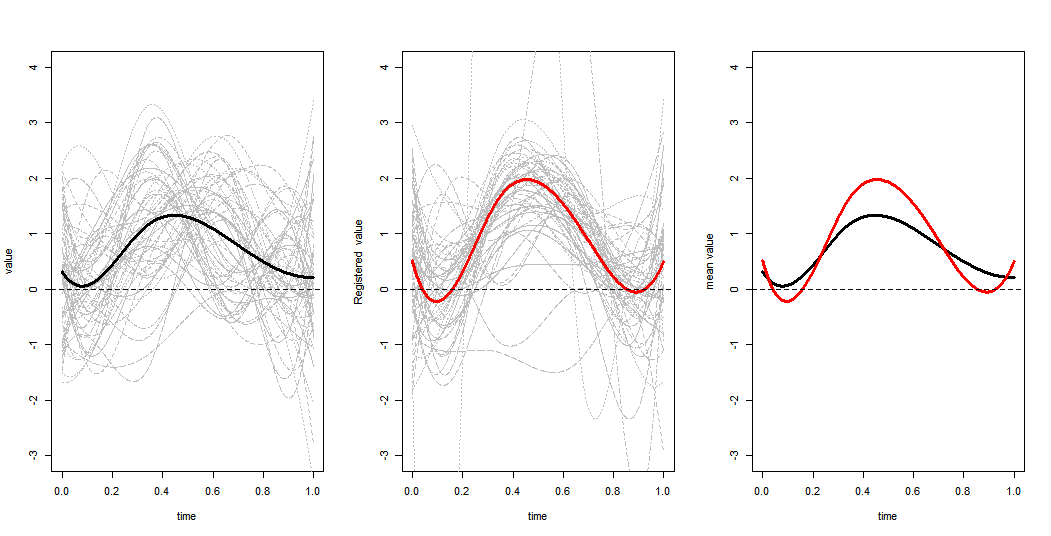
\includegraphics[height=7cm]{matern_align_compare.png}
    \caption{Mat\'{e}rn process: before \& after alignment}
\end{figure}
Each curve on plots indicates,
\begin{itemize}
    \item{\textbf{left:} Before alignment. \\
    gray: Using 6 b-spline basis, get each curve corresponds to each process generated at above.\\
    bold black: the mean function of fitted curves before alignment.}
    \item{\textbf{middle:} After alignment. \\
    gray: aligned curves for fitted ones using 6 b-spline basis to each process.\\
    bold red: the mean function of aligned curves.}
    \item{\textbf{right:} plot only mean curves.\\
    bold black: the mean function of unaligned curves.\\
    bold red: the mean function of aligned curves.}
\end{itemize}


Because we generated processes through transforming Mat\'{e}rn processes of same covariance structure 
by 2 bump function whose shapes are same except only location, the effect of the alignment is enormous.
The gray curves of aligned plot are adjusted to move with harmony, up and down at respective neighborhoods on x-axis for most observations
comparing with unaligned's gray curves. And as a result of alignment, a the mean curve of aligned one is more explanatory than unaligned one, 
especially showing higher amplitude(function value) which reflects each sample (gray) curve more exactly.


\newpage
\subsection*{(c) Carry out an FPCA with one PC on the unaligned and aligned curves separately. 
For each, do a simple linear regression of the score onto a dummy variable (coded 0/1) 
indicating which type of mean the function had (i.e. is it from the first or second half of the sample). 
Calculate a p-value to determine if the estimated slope parameters you get are significant. 
Compare with the aligned and unaligned curves. What did aligning do to the p-value? 
You may want to rerun your simulations a few times to see how the p-values change.}

Execute below code for doing pca with an one component and calculating p-value after least-square estimation of score onto group category variable.
\begin{Rcode}
    \begin{verbatim}
#pca
adjMtSample.f.pca = pca.fd(adjMtSample.f, nharm=1)
adjMtSample.f.reg.pca = pca.fd(adjMtSample.f.reg$regfd, nharm=1)

#pca component plot
par(mfrow=c(1,1))
plot(adjMtSample.f.pca$harmonics, ylim=c(-3,4))
plot(adjMtSample.f.reg.pca$harmonics, col='red', add=T)
    \end{verbatim}
\end{Rcode}

Firstly, we examine the results of PCA for each case. Below is plot of first eigenfunction of each aligned and unaligned case.

\begin{figure}[hh]
    \centering
    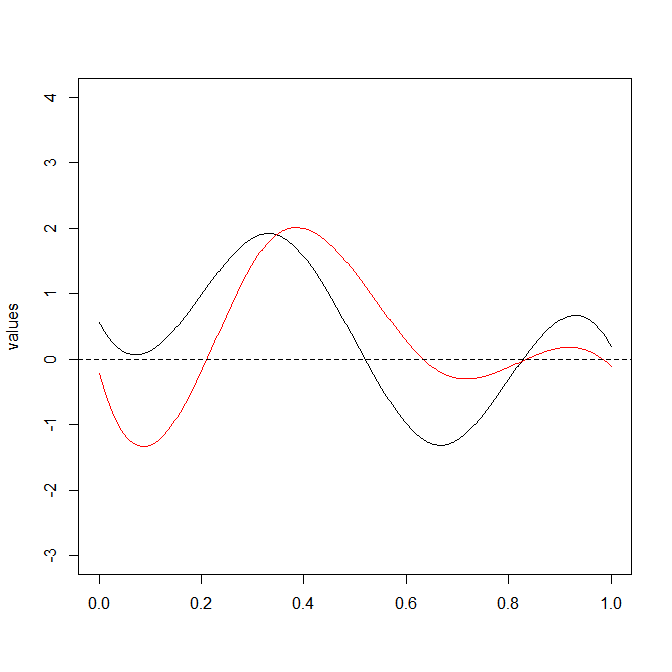
\includegraphics[height=8cm]{matern_pca_component.png}
    \caption{Mat\'{e}rn process: PCA before \& after alignment \\
    black : 1st component of pca of before alignment case\\
    red : 1st component of pca of after alignment case}
\end{figure}

Observe that, by alignment, the component moves to right, direction to the total mean. It is effect of continuous registration,
since the method aligns curves with the mean's location.

We can also get the proportion of explained variation by the first component in R, for each case.
\begin{console}
    \begin{verbatim}
> adjMtSample.f.pca$varprop
[1] 0.3593796
> adjMtSample.f.reg.pca$varprop
[1] 0.7315676
    \end{verbatim}
\end{console}
The proportion are doubled! It consists the big effect of alignment which we discover when examine mean curves. 
(In fact, the result - increased variance proportion - is NOT observed all simulation cases. It depends on simulated
random processes' degree of similarity of general shapes (when each process path are more similar, more improvement!), 
so in general, if we simulate with other random-seed value or simply repeat simulation more times, the size of improvement does NOT reach
to double through alignment, even there can be cases for decrease after alignment.)

In succession, I will do least square fit of score onto group index. 
For this work, I will make the dummy variable, call simple regression code to each case,
and plot the result and get p-value of slope following the direction of problem.
Run below code.
\begin{Rcode}
    \begin{verbatim}
dummy_var = c(rep(0,num.sample/2),rep(1,num.sample/2))
un_align_score = adjMtSample.f.pca$score
align_score = adjMtSample.f.reg.pca$score

par(mfrow=c(1,2))
lm1_unaligned= lm(un_align_score ~ dummy_var)
plot(dummy_var, un_align_score, ylim=c(-1.5, 1))
abline(lm1_unaligned$coefficient, col='red')
summary(lm1_unaligned)

lm2_aligned= lm(align_score ~ dummy_var)
plot(dummy_var, align_score, ylim=c(-1.5, 1))
abline(lm2_aligned$coefficient, col='red')
summary(lm2_aligned)        
    \end{verbatim}
\end{Rcode}

The results are,

\begin{figure}[hh]
    \centering
    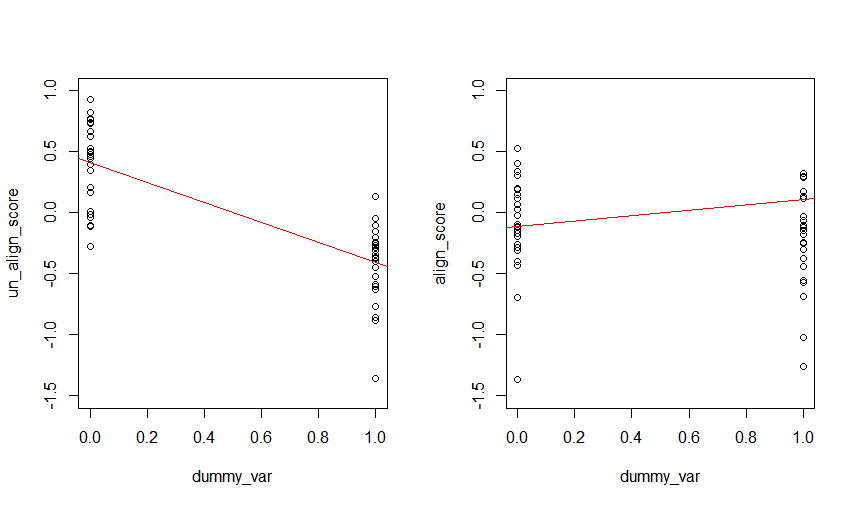
\includegraphics[height=6.8cm]{matern_score_reg.png}
    \caption{Mat\'{e}rn process: regression of score onto group dummy variable\\
    left: before alignment, right: after alignment
    0: first 25 group, 1: last 25 group
    }
\end{figure}
\begin{console}
    \begin{verbatim}
> summary(lm1_unaligned)
Call:
lm(formula = un_align_score ~ dummy_var)
Residuals:
     Min       1Q   Median       3Q      Max
-0.94443 -0.20165  0.06072  0.24753  0.54723
Coefficients:
            Estimate Std. Error t value Pr(>|t|)
(Intercept)  0.40993    0.06706   6.113 1.68e-07 ***
dummy_var   -0.81987    0.09483  -8.646 2.37e-11 ***
---
Signif. codes:  0 '***' 0.001 '**' 0.01 '*' 0.05 '.' 0.1 ' ' 1
Residual standard error: 0.3353 on 48 degrees of freedom
Multiple R-squared:  0.6089,    Adjusted R-squared:  0.6008
F-statistic: 74.75 on 1 and 48 DF,  p-value: 2.371e-11

> summary(lm2_aligned)
Call:
lm(formula = align_score ~ dummy_var)
Residuals:
    Min      1Q  Median      3Q     Max
-1.3657 -0.3425 -0.1131  0.1634  7.6486
Coefficients:
            Estimate Std. Error t value Pr(>|t|)
(Intercept)  -0.1077     0.2387  -0.451    0.654
dummy_var     0.2154     0.3375   0.638    0.526
Residual standard error: 1.193 on 48 degrees of freedom
Multiple R-squared:  0.008415,  Adjusted R-squared:  -0.01224
F-statistic: 0.4074 on 1 and 48 DF,  p-value: 0.5263
    \end{verbatim}
\end{console}

We can observe that,
\begin{itemize}
    \item {Before alignment, the slope value of the regression result is significantly NOT 0 
    since the p-value of slope coefficient are 2.37e-11, very small value.}
    \item {After alignment, the p-value corresponds to slope coefficient is 0.526, so we can make a
    conclusion that the slope is statistically 0.
    }
\end{itemize}

So, in unaligned case, the scores have different level depending on that the sample belongs to which group,
but in aligned case, this phenomenon are not represented.
It may be able to be explained by below intuition.

\begin{itemize}
    \item{For case of before alignment, although there were 2 types of shape of processes, we use only an 1 component.
    So in fitting process using the eigenfunction to each for original process (or similarly curve fitted by b-spline basis earlier),
    naturally the score - the scalar value multiplied to the component to make nearest fit to each observation - are 2-grouped. 
    And the result is presented by significant slope value with low p-value in above regression.}
    \item{While, for the case of after alignment, all (or most) fitted curves by b-spline basis are 
    have similar shape by alignment step. So in fitting process using an eigenfunction,
    all multipliers of the function to make nearest fit become having similar values.
    And it makes the result that the coefficient of dummy variable is NOT significant with high p-value in above regression.}
\end{itemize}




\subsection*{(d) Come up with one potential setting/application 
where you might lose something if you align. Make up whatever scenario you like, but think it through.}

As we see above example simulation, the alignment procesure deletes some information about location which
curves moves specially on some time which follows respectively tuned clock for each sample but the moving shapes are similar for each observation.
Thus, for perpose of inference, if the triggered time at which value starts to move specifically is important information, We SHOULD NOT do alignment procedure.


A toy example situration is here:\\
We want to know the distribution of age that boys start to grow faster in adolescence period 
by begining a secondary sexual characteristics. And we get some samples that form of functional-data.

In this case, if we align the curves, we lose information about 'starting age' of most boys, instead
we unintentionally emphasize some unnecessary information like a mean growing length of them.
Consquently, we will fail to infer properly from the data contextually, cannot achieve the purpose - getting distribution of starting age.


\end{document}
